\problemname{Cheaper Drink}

%\illustration{.3}{Yardley_Wood.jpg}{A wall calendar displaying the date 5 OCT. Image source: Yardley Wood Bus Garage - Open Day - signs - date - Oct 05.  Author:	Elliott Brown from Birmingham, United Kingdom. Wikimedia Commons.}

Instead of worrying about the current hyperinflation you decide to go down to the local bar and have a drink.

The prices at the bar are displayed using magnetic signs with numbers printed on them, with each magnet showing one or more digits.
For instance, the price of 1106 megacredits is displayed like this:

\medskip
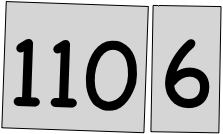
\includegraphics[width = 2cm]{img/from.png}

While the bartender is busy serving the next customer, you have just enough time to rearrange the price of your favourite beverage to make it as cheap as possible.
But be quick about it!

Individual magnets can be moved around in any order and turned upside-down.
The numbers are shown in a script that makes it difficult for the bartender to distinguish 0, 1, and 8 from their upside-down counterpart.
Moreover, 6 and 9 look the same when one is turned upside-down.
The example price above could be made almost ten times cheaper by turning the first magnet:

\medskip
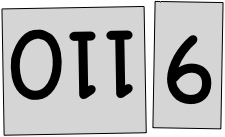
\includegraphics[width = 2cm]{img/to.png}

You have to use all the magnets, otherwise the bartender will immediately suspect foul play.

\section*{Input}

On the first line, the number $n$ of magnets, with $1\in\{1,\ldots, 1\,000\}$.
On each of the following $n$ lines, exactly one sequence $m_i$ of digits describing the $i$th magnet.
Each magnet $m_i$ for $i\in \{1,\ldots, n\}$ consists of at least one and at most 10 digits from $0$, $1$, $\ldots$, $9$.
The price currently displayed on the bar is the integer described by the juxtaposition $m_1\cdots m_n$ of the magnets in the order they are given, from left to right.
Note that a magnet can be all $0$s, even though the current price at the bar, alas!, is certainly not.

\section*{Output}

A single line containing the cheapest price formed by the magnets $m_1,\ldots,m_n$, rearranged in any order, and each of them possibly turned upside-down.
